
%% bare_conf.tex
%% V1.4b
%% 2015/08/26
%% by Michael Shell
%% See:
%% http://www.michaelshell.org/
%% for current contact information.
%%
%% This is a skeleton file demonstrating the use of IEEEtran.cls
%% (requires IEEEtran.cls version 1.8b or later) with an IEEE
%% conference paper.
%%
%% Support sites:
%% http://www.michaelshell.org/tex/ieeetran/
%% http://www.ctan.org/pkg/ieeetran
%% and
%% http://www.ieee.org/

%%*************************************************************************
%% Legal Notice:
%% This code is offered as-is without any warranty either expressed or
%% implied; without even the implied warranty of MERCHANTABILITY or
%% FITNESS FOR A PARTICULAR PURPOSE! 
%% User assumes all risk.
%% In no event shall the IEEE or any contributor to this code be liable for
%% any damages or losses, including, but not limited to, incidental,
%% consequential, or any other damages, resulting from the use or misuse
%% of any information contained here.
%%
%% All comments are the opinions of their respective authors and are not
%% necessarily endorsed by the IEEE.
%%
%% This work is distributed under the LaTeX Project Public License (LPPL)
%% ( http://www.latex-project.org/ ) version 1.3, and may be freely used,
%% distributed and modified. A copy of the LPPL, version 1.3, is included
%% in the base LaTeX documentation of all distributions of LaTeX released
%% 2003/12/01 or later.
%% Retain all contribution notices and credits.
%% ** Modified files should be clearly indicated as such, including  **
%% ** renaming them and changing author support contact information. **
%%*************************************************************************


% *** Authors should verify (and, if needed, correct) their LaTeX system  ***
% *** with the testflow diagnostic prior to trusting their LaTeX platform ***
% *** with production work. The IEEE's font choices and paper sizes can   ***
% *** trigger bugs that do not appear when using other class files.       ***                          ***
% The testflow support page is at:
% http://www.michaelshell.org/tex/testflow/



\documentclass[conference]{IEEEtran}
% Some Computer Society conferences also require the compsoc mode option,
% but others use the standard conference format.
%
% If IEEEtran.cls has not been installed into the LaTeX system files,
% manually specify the path to it like:
% \documentclass[conference]{../sty/IEEEtran}





% Some very useful LaTeX packages include:
% (uncomment the ones you want to load)


% *** MISC UTILITY PACKAGES ***
%
%\usepackage{ifpdf}
% Heiko Oberdiek's ifpdf.sty is very useful if you need conditional
% compilation based on whether the output is pdf or dvi.
% usage:
% \ifpdf
%   % pdf code
% \else
%   % dvi code
% \fi
% The latest version of ifpdf.sty can be obtained from:
% http://www.ctan.org/pkg/ifpdf
% Also, note that IEEEtran.cls V1.7 and later provides a builtin
% \ifCLASSINFOpdf conditional that works the same way.
% When switching from latex to pdflatex and vice-versa, the compiler may
% have to be run twice to clear warning/error messages.






% *** CITATION PACKAGES ***
%
%\usepackage{cite}
% cite.sty was written by Donald Arseneau
% V1.6 and later of IEEEtran pre-defines the format of the cite.sty package
% \cite{} output to follow that of the IEEE. Loading the cite package will
% result in citation numbers being automatically sorted and properly
% "compressed/ranged". e.g., [1], [9], [2], [7], [5], [6] without using
% cite.sty will become [1], [2], [5]--[7], [9] using cite.sty. cite.sty's
% \cite will automatically add leading space, if needed. Use cite.sty's
% noadjust option (cite.sty V3.8 and later) if you want to turn this off
% such as if a citation ever needs to be enclosed in parenthesis.
% cite.sty is already installed on most LaTeX systems. Be sure and use
% version 5.0 (2009-03-20) and later if using hyperref.sty.
% The latest version can be obtained at:
% http://www.ctan.org/pkg/cite
% The documentation is contained in the cite.sty file itself.






% *** GRAPHICS RELATED PACKAGES ***
%
\ifCLASSINFOpdf
  \usepackage[pdftex]{graphicx}
  % declare the path(s) where your graphic files are
  % \graphicspath{{../pdf/}{../jpeg/}}
  % and their extensions so you won't have to specify these with
  % every instance of \includegraphics
  % \DeclareGraphicsExtensions{.pdf,.jpeg,.png}
\else
  % or other class option (dvipsone, dvipdf, if not using dvips). graphicx
  % will default to the driver specified in the system graphics.cfg if no
  % driver is specified.
  % \usepackage[dvips]{graphicx}
  % declare the path(s) where your graphic files are
  % \graphicspath{{../eps/}}
  % and their extensions so you won't have to specify these with
  % every instance of \includegraphics
  % \DeclareGraphicsExtensions{.eps}
\fi

% *** MATH PACKAGES ***
%
\usepackage{amsmath}
% A popular package from the American Mathematical Society that provides
% many useful and powerful commands for dealing with mathematics.
%
% Note that the amsmath package sets \interdisplaylinepenalty to 10000
% thus preventing page breaks from occurring within multiline equations. Use:
%\interdisplaylinepenalty=2500
% after loading amsmath to restore such page breaks as IEEEtran.cls normally
% does. amsmath.sty is already installed on most LaTeX systems. The latest
% version and documentation can be obtained at:
% http://www.ctan.org/pkg/amsmath





% *** SPECIALIZED LIST PACKAGES ***
%
%\usepackage{algorithmic}
% algorithmic.sty was written by Peter Williams and Rogerio Brito.
% This package provides an algorithmic environment fo describing algorithms.
% You can use the algorithmic environment in-text or within a figure
% environment to provide for a floating algorithm. Do NOT use the algorithm
% floating environment provided by algorithm.sty (by the same authors) or
% algorithm2e.sty (by Christophe Fiorio) as the IEEE does not use dedicated
% algorithm float types and packages that provide these will not provide
% correct IEEE style captions. The latest version and documentation of
% algorithmic.sty can be obtained at:
% http://www.ctan.org/pkg/algorithms
% Also of interest may be the (relatively newer and more customizable)
% algorithmicx.sty package by Szasz Janos:
% http://www.ctan.org/pkg/algorithmicx




% *** ALIGNMENT PACKAGES ***
%
%\usepackage{array}
% Frank Mittelbach's and David Carlisle's array.sty patches and improves
% the standard LaTeX2e array and tabular environments to provide better
% appearance and additional user controls. As the default LaTeX2e table
% generation code is lacking to the point of almost being broken with
% respect to the quality of the end results, all users are strongly
% advised to use an enhanced (at the very least that provided by array.sty)
% set of table tools. array.sty is already installed on most systems. The
% latest version and documentation can be obtained at:
% http://www.ctan.org/pkg/array


% IEEEtran contains the IEEEeqnarray family of commands that can be used to
% generate multiline equations as well as matrices, tables, etc., of high
% quality.




% *** SUBFIGURE PACKAGES ***
%\ifCLASSOPTIONcompsoc
%  \usepackage[caption=false,font=normalsize,labelfont=sf,textfont=sf]{subfig}
%\else
%  \usepackage[caption=false,font=footnotesize]{subfig}
%\fi
% subfig.sty, written by Steven Douglas Cochran, is the modern replacement
% for subfigure.sty, the latter of which is no longer maintained and is
% incompatible with some LaTeX packages including fixltx2e. However,
% subfig.sty requires and automatically loads Axel Sommerfeldt's caption.sty
% which will override IEEEtran.cls' handling of captions and this will result
% in non-IEEE style figure/table captions. To prevent this problem, be sure
% and invoke subfig.sty's "caption=false" package option (available since
% subfig.sty version 1.3, 2005/06/28) as this is will preserve IEEEtran.cls
% handling of captions.
% Note that the Computer Society format requires a larger sans serif font
% than the serif footnote size font used in traditional IEEE formatting
% and thus the need to invoke different subfig.sty package options depending
% on whether compsoc mode has been enabled.
%
% The latest version and documentation of subfig.sty can be obtained at:
% http://www.ctan.org/pkg/subfig




% *** FLOAT PACKAGES ***
%
%\usepackage{fixltx2e}
% fixltx2e, the successor to the earlier fix2col.sty, was written by
% Frank Mittelbach and David Carlisle. This package corrects a few problems
% in the LaTeX2e kernel, the most notable of which is that in current
% LaTeX2e releases, the ordering of single and double column floats is not
% guaranteed to be preserved. Thus, an unpatched LaTeX2e can allow a
% single column figure to be placed prior to an earlier double column
% figure.
% Be aware that LaTeX2e kernels dated 2015 and later have fixltx2e.sty's
% corrections already built into the system in which case a warning will
% be issued if an attempt is made to load fixltx2e.sty as it is no longer
% needed.
% The latest version and documentation can be found at:
% http://www.ctan.org/pkg/fixltx2e


%\usepackage{stfloats}
% stfloats.sty was written by Sigitas Tolusis. This package gives LaTeX2e
% the ability to do double column floats at the bottom of the page as well
% as the top. (e.g., "\begin{figure*}[!b]" is not normally possible in
% LaTeX2e). It also provides a command:
%\fnbelowfloat
% to enable the placement of footnotes below bottom floats (the standard
% LaTeX2e kernel puts them above bottom floats). This is an invasive package
% which rewrites many portions of the LaTeX2e float routines. It may not work
% with other packages that modify the LaTeX2e float routines. The latest
% version and documentation can be obtained at:
% http://www.ctan.org/pkg/stfloats
% Do not use the stfloats baselinefloat ability as the IEEE does not allow
% \baselineskip to stretch. Authors submitting work to the IEEE should note
% that the IEEE rarely uses double column equations and that authors should try
% to avoid such use. Do not be tempted to use the cuted.sty or midfloat.sty
% packages (also by Sigitas Tolusis) as the IEEE does not format its papers in
% such ways.
% Do not attempt to use stfloats with fixltx2e as they are incompatible.
% Instead, use Morten Hogholm'a dblfloatfix which combines the features
% of both fixltx2e and stfloats:
%
% \usepackage{dblfloatfix}
% The latest version can be found at:
% http://www.ctan.org/pkg/dblfloatfix




% *** PDF, URL AND HYPERLINK PACKAGES ***
%
%\usepackage{url}
% url.sty was written by Donald Arseneau. It provides better support for
% handling and breaking URLs. url.sty is already installed on most LaTeX
% systems. The latest version and documentation can be obtained at:
% http://www.ctan.org/pkg/url
% Basically, \url{my_url_here}.




% *** Do not adjust lengths that control margins, column widths, etc. ***
% *** Do not use packages that alter fonts (such as pslatex).         ***
% There should be no need to do such things with IEEEtran.cls V1.6 and later.
% (Unless specifically asked to do so by the journal or conference you plan
% to submit to, of course. )


% correct bad hyphenation here
\hyphenation{op-tical net-works semi-conduc-tor}


\begin{document}
%
% paper title
% Titles are generally capitalized except for words such as a, an, and, as,
% at, but, by, for, in, nor, of, on, or, the, to and up, which are usually
% not capitalized unless they are the first or last word of the title.
% Linebreaks \\ can be used within to get better formatting as desired.
% Do not put math or special symbols in the title.
\title{Digital Predistortion with Low Precision ADCs}


% author names and affiliations
% use a multiple column layout for up to three different
% affiliations
%\author{\IEEEauthorblockN{Chance Tarver}
%\IEEEauthorblockA{Department of Electrical and\\Computer Engineering\\
%Rice University\\
%Atlanta, Georgia 30332--0250\\
%Email:tarver@rice.edu}
%\and
%\IEEEauthorblockN{Joe Cavallaro}
%\IEEEauthorblockA{Twentieth Century Fox\\
%Springfield, USA\\
%Email: homer@thesimpsons.com}
%}

% conference papers do not typically use \thanks and this command
% is locked out in conference mode. If really needed, such as for
% the acknowledgment of grants, issue a \IEEEoverridecommandlockouts
% after \documentclass

% for over three affiliations, or if they all won't fit within the width
% of the page, use this alternative format:
% 
\author{
\IEEEauthorblockN{
Chance Tarver \ and \
Joseph R. Cavallaro}
\IEEEauthorblockA{
Department of Electrical and Computer Engineering, 
Rice University, Houston, TX \\ Email: tarver@rice.edu  cavallar@rice.edu}}



% use for special paper notices
%\IEEEspecialpapernotice{(Invited Paper)}

% make the title area
\maketitle

% As a general rule, do not put math, special symbols or citations
% in the abstract
\begin{abstract}
Digital Predistortion (DPD) is a popular technique for linearizing a power amplifier (PA) to help reduce the spurious emissions and spectral regrowth. DPD requires the learning of the inverse PA nonlinearities by training on the output of the PA. In practical systems, the analog output of the PA will have to go through an analog-to-digital converter (ADC) so that training can be done on a digital processor. The quantization degrades signal quality and may limit the performance of a DPD learning algorithm. However, a lower resolution ADC may cost less and allow for less computational complexity in the digital processing. 
We study this trade-off to try to find how much precision is needed in DPD systems and discover that for a full-band DPD as few as 6 bits can reliably be used. 
For sub-band DPD, a single bit ADC can be used. 
\end{abstract}

% no keywords




% For peer review papers, you can put extra information on the cover
% page as needed:
% \ifCLASSOPTIONpeerreview
% \begin{center} \bfseries EDICS Category: 3-BBND \end{center}
% \fi
%
% For peerreview papers, this IEEEtran command inserts a page break and
% creates the second title. It will be ignored for other modes.
%\IEEEpeerreviewmaketitle


\section{Introduction}
The power amplifier (PA) is a component of wireless systems that has a nonlinear transfer function. 
The nonlinearities are undesirable in that they lead to distortions such as spectral regrowth around the main carriers and intermodulation distortions (IMDs) in scenarios with multiple, noncontiguous carriers such as carrier aggregation (CA) in LTE-Advanced. 
This is exacerbated in modern, multi-carrier modulations such as OFDMA which have a high peak-to-average power ratio (PAPR). 

Digital predistortion (DPD) is a method for linearizing a power amplifier (PA). 
With DPD, the nonlinearities are estimated so that they can be corrected before the PA with their inverse.
To do this, we must train our predistorter by observing the signal after the PA.
In practical situations, we need a feedback path after the PA that has a downconverter and an ADC.
Typically, DPD bandwidth is five times the signal bandwidth  \cite{Katz2016}. Hence, for wide bandwidth signals, the sampling rate of the ADC must be fast. 

In mobile applications where power and cost are a concern, one option for reducing the complexity of the system is to use a low precision ADC. 
By reducing the precision, the DPD algrothim can be performed with shorter word lengths which would save area and power in an implementation. 
Low precision ADCs often consume less power and support faster sampling rates than higher precision devices \cite{Walden99}. Moreover, these ADC are often cheaper. 

For these reasons, the use of low precision ADCs is being considered in multiple emerging areas of communications. For example, in massive MIMO resolutions as low as a single bit are being considered to help alleviate the data throughput requirements when hundreds of antennas are being used simultaneously \cite{MIMOAdcs}. In mmWave, there are large bandwidths available that could enable fast data rates. This necessitates the use of ADCs with fast sampling rates. Again, low-precision ADCs are being considered for this application to reduce the system complexity and power requirements \cite{Heath2015}. 

In this paper, we test the performance of our previous DPD solutions for varying ADC precision. 
By doing so, we alter the resolution of the feedback path to the DPD learning. 
As we remove bits, we increase quantization noise which we expect to limit performance. 
What we find is that a significant number of bits can be removed before there is a significant impact on performance.

The paper is organized as follows. 
Section II presents a simulation where we reduce the precision on a full-band DPD. 
In Section III, we repeat the simulation with a sub-band DPD. 
We then conclude the paper in Section IV.

\section{Full-Band DPD}

\begin{figure}[]
	\centering
	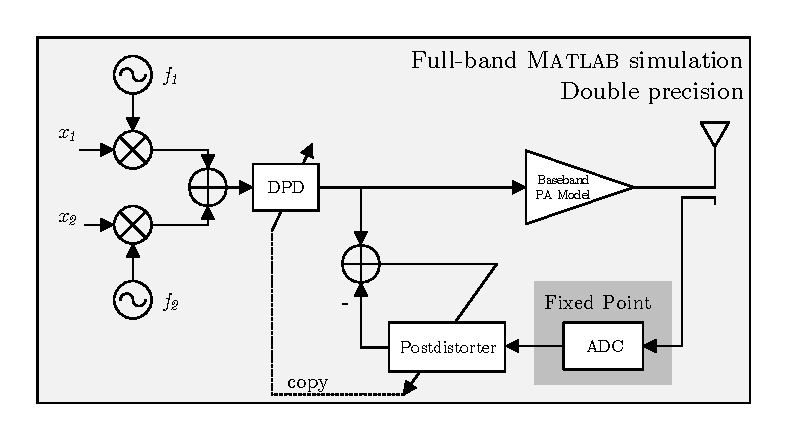
\includegraphics[width=\columnwidth]{FullBandIndirect}
	\caption{Block diagram of the full-band DPD simulation performed. The signal generation, amplification, indirect DPD learning, and DPD application are performed with double precision in \textsc{Matlab}. We emulate an ADC by quantizing the feedback from the PA to the DPD learning.}
	\label{block}
\end{figure}

Most DPD is a variation of what we refer to as full-band DPD where the entire transmit band near the main carriers is linearized. 
This can reduce the magnitude of multiple spurious emissions such as the third and fifth intermodulation products and the spectral regrowth around the main carriers. 
However, this comes with a considerable computational complexity especially as the spacing between the carriers becomes large \cite{TMTT_SubbandDPD} which also has the negative effect of increasing power consumption and cost in the ADC.

A block diagram of the simulation is shown in Figure \ref{block}. Currently, all computation is done in double precision. However, at the feedback input to the DPD learning, we quantize using the fixed-point toolbox. Word lengths are varied from an unquantified sixty-four bit double all the way to two bits. When we perform the DPD algorithm where the feedback into the DPD learning block is the full, double-precision values computed by \textsc{Matlab}, we get suppression shown by the solid blue curve in Figure \ref{fullbandpsd}. We then use signed, fixed-point representation. This introduces quantization noise and degrades the performance. However, for as low as 6-bit ADC, the performance degradation is mostly insignificant. For example, there is only a 2 dB difference in suppression on the right-hand IM3 spur. The 4-bit ADC still suppress throughout the spectrum, but there is a significant performance degradation (14 dB on the right-hand IM3). 

Using a previously developed DPD system \cite{Li2016GPU} we illustrate the effect of quantization in Figure \ref{fullbandpsd}. 
Here, we have two noncontiguous signals like what may be found in LTE-Advanced carrier aggregation. They are each 5 MHz in bandwidth. 
They are broadcast through a fifth-order, nonlinear PA model with memory effects implemented in \textsc{Matlab}. 
Intermodulation occurs and introduces large spurious emissions through the nearby spectrum as seen by the black curve.

Here, we are limited by the available dynamic range of the low precision. 
As we reduce the bits, the noise floor of the feedback raises due to quantization noise. 
The ADC becomes saturated by the power of the main carriers and simply can not see the relatively low power signals of the spurious emissions. 


\begin{figure}[]
\centering
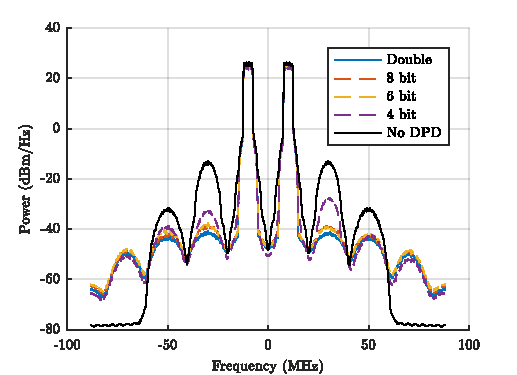
\includegraphics[]{FullBandPSD}
\caption{PSD output when performing full-band DPD on a scenario with two, noncontiguous, 5 MHz LTE uplink carriers with a low precision ADC feedback path. Here, performance for the 8 bit and 6 bit ADCs are similar with about 2 dB less IM3 suppression when compared to the double-precision PA simulation.}
\label{fullbandpsd}
\end{figure}


\section{Sub-Band DPD}
An alternative to the full-band DPD is what the authors refer to as sub-band DPD. 
With this method, one targets specific sub-bands such as prominent intermodulation products for suppression. 
This has the effect of drastically reducing sample rates which in turn reduces the running complexity of the algorithm. 
This method also provides freedom in the sense that specific sub-bands can be targeted as needed. 

Using a previously developed sub-band DPD system \cite{TMTT_SubbandDPD} we illustrate the effect of quantization in Figure \ref{subbandpsd}. Here, we have two noncontiguous signals like what may be found in LTE-Advanced carrier aggregation. They are each 1.4 MHz in bandwidth. They are broadcast through a ninth-order, nonlinear PA model implemented in \textsc{Matlab}. 
Intermodulation occurs and introduces large spurious emissions through the nearby spectrum as seen by the black curve. We use the sub-band DPD method to target the right-hand, third-order intermodulation spurious emission.

When using the sub-band method, it is not necessary to receive the main carriers in the feedback path.
Instead, a sub-band DPD can be designed as follows. 
The RF downconverter can be tuned to the specific frequency of a problematic spurious emission.
Then, an analog low-pass filter (LPF) can be used for anti-aliasing and attenuation of the higher-power main carriers. 
By doing this, we can better use the low dynamic-range available when using a low-precision ADC to receive just the spurious emission.
This will provide better performance in the DPD learning algorithm. 
The block diagram of the proposed system and how it was simulated is shown in Figure \ref{block2}.

\begin{figure}[]
	\centering
	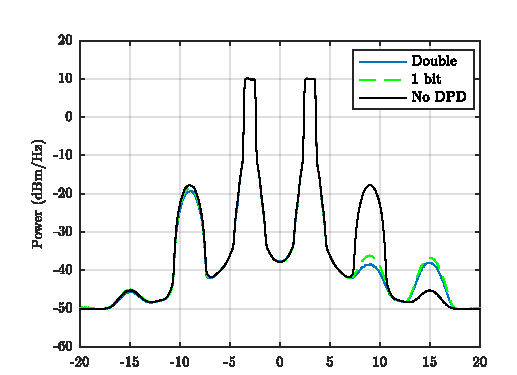
\includegraphics[]{SubBandPSD}
	\caption{PSD output when performing sub-band DPD on a scenario with two, noncontiguous, 1.4 MHz LTE uplink carriers with a 1 bit ADC feedback path. Here, performance for the single bit observations has about 2 dB less IM3 suppression when compared to the double-precision PA simulation. }
	\label{subbandpsd}
\end{figure}

\begin{figure}[]
	\centering
	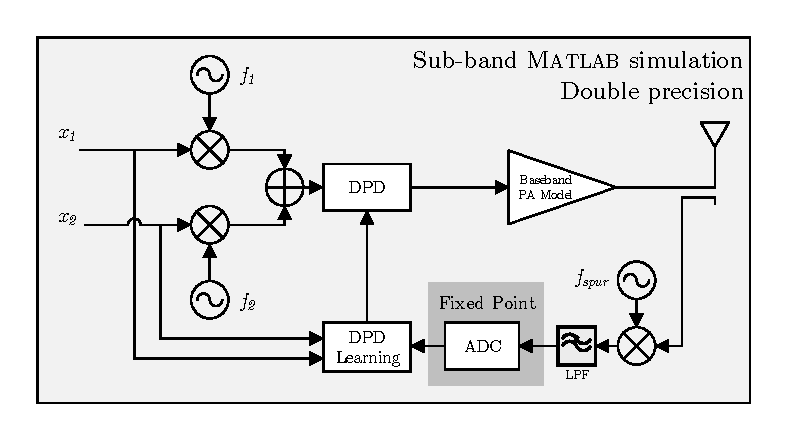
\includegraphics[width=\columnwidth]{SubBand}
	\caption{Block diagram of the sub-band DPD simulation performed. Here, we tune the feedback receiver to the frequency of the spur and pass it through a low-pass filter. The frequency shift, low-pass filtering, signal generation, amplification, DPD learning, and DPD application are performed with double precision in \textsc{Matlab}. We emulate an ADC by quantizing the feedback from the PA to the DPD learning.}
	\label{block2}
\end{figure}

 When we perform the third-order DPD algorithm where the feedback into the DPD learning block is the full, double-precision values computed by \textsc{Matlab}, we get suppression shown by the solid blue curve in Figure \ref{subbandpsd}. We then use \textsc{Matlab}'s fixed point toolbox to convert the values to a signed, fixed-point representation. This introduces quantization noise and degrades the performance. 
 However, for as low as a single-bit ADC, the performance degradation is mostly insignificant. For example, there is only a 2 dB difference in suppression on the right-hand IM3 spur. 
 
 This creates an exciting opportunity for reducing the complexity of the hardware necessary for a system using the sub-band DPD algorithm. 
 The RF downconverter can be a lower-cost, smaller-bandwidth device since only a sub-band needs to be used for training.
 The ADC can be replaced by a comparator.
 This has the effect of reducing area and power overhead which is attractive for mobile devices.
 
 The algorithmic complexity can also be reduced. The sub-band DPD learning algorithm is accomplished in \cite{TMTT_SubbandDPD} via an LMS adaptive training. A version of this is shown below,
 \begin{align}
 \alpha^*(n+1) &= \alpha^*(n) - \frac{\mu}{|u(n)||^2 + C} e^*(n) u(n).
 \label{eq:NLMS_Update_memory}
 \end{align}
Here $\alpha$ is the DPD coefficient,
$e(n)$ is the error signal vector of a spur at the PA output, $u(n)$ is the LMS reference signal, $\mu$ is the LMS learning rate, and $n$ denotes the sample index. 
The DPD application is achieved by adding a term to the PA input,
\begin{align}
\tilde{x}(n) &=  x(n) + \left[\alpha \star u(n) \right] e^{j 2\pi \frac{f_{spur}}{f_s} n}.
\end{align}

The complex multiplication of the error signal by the reference signal in Equation \ref{eq:NLMS_Update_memory}, can be simplified when the error signal is only 1-bit. The multiplication becomes sign changes and additions to $u(n)$. This reduces the complexity which helps simplify the implementation of the learning algorithm. 


%\section{WARPLab Testing}
% An example of a floating figure using the graphicx package.
% Note that \label must occur AFTER (or within) \caption.
% For figures, \caption should occur after the \includegraphics.
% Note that IEEEtran v1.7 and later has special internal code that
% is designed to preserve the operation of \label within \caption
% even when the captionsoff option is in effect. However, because
% of issues like this, it may be the safest practice to put all your
% \label just after \caption rather than within \caption{}.
%
% Reminder: the "draftcls" or "draftclsnofoot", not "draft", class
% option should be used if it is desired that the figures are to be
% displayed while in draft mode.
%
%\begin{figure}[!t]
%\centering
%\includegraphics[width=2.5in]{myfigure}
% where an .eps filename suffix will be assumed under latex, 
% and a .pdf suffix will be assumed for pdflatex; or what has been declared
% via \DeclareGraphicsExtensions.
%\caption{Simulation results for the network.}
%\label{fig_sim}
%\end{figure}

% Note that the IEEE typically puts floats only at the top, even when this
% results in a large percentage of a column being occupied by floats.


% An example of a double column floating figure using two subfigures.
% (The subfig.sty package must be loaded for this to work.)
% The subfigure \label commands are set within each subfloat command,
% and the \label for the overall figure must come after \caption.
% \hfil is used as a separator to get equal spacing.
% Watch out that the combined width of all the subfigures on a 
% line do not exceed the text width or a line break will occur.
%
%\begin{figure*}[!t]
%\centering
%\subfloat[Case I]{\includegraphics[width=2.5in]{box}%
%\label{fig_first_case}}
%\hfil
%\subfloat[Case II]{\includegraphics[width=2.5in]{box}%
%\label{fig_second_case}}
%\caption{Simulation results for the network.}
%\label{fig_sim}
%\end{figure*}
%
% Note that often IEEE papers with subfigures do not employ subfigure
% captions (using the optional argument to \subfloat[]), but instead will
% reference/describe all of them (a), (b), etc., within the main caption.
% Be aware that for subfig.sty to generate the (a), (b), etc., subfigure
% labels, the optional argument to \subfloat must be present. If a
% subcaption is not desired, just leave its contents blank,
% e.g., \subfloat[].


% An example of a floating table. Note that, for IEEE style tables, the
% \caption command should come BEFORE the table and, given that table
% captions serve much like titles, are usually capitalized except for words
% such as a, an, and, as, at, but, by, for, in, nor, of, on, or, the, to
% and up, which are usually not capitalized unless they are the first or
% last word of the caption. Table text will default to \footnotesize as
% the IEEE normally uses this smaller font for tables.
% The \label must come after \caption as always.
%
%\begin{table}[!t]
%% increase table row spacing, adjust to taste
%\renewcommand{\arraystretch}{1.3}
% if using array.sty, it might be a good idea to tweak the value of
% \extrarowheight as needed to properly center the text within the cells
%\caption{An Example of a Table}
%\label{table_example}
%\centering
%% Some packages, such as MDW tools, offer better commands for making tables
%% than the plain LaTeX2e tabular which is used here.
%\begin{tabular}{|c||c|}
%\hline
%One & Two\\
%\hline
%Three & Four\\
%\hline
%\end{tabular}
%\end{table}


% Note that the IEEE does not put floats in the very first column
% - or typically anywhere on the first page for that matter. Also,
% in-text middle ("here") positioning is typically not used, but it
% is allowed and encouraged for Computer Society conferences (but
% not Computer Society journals). Most IEEE journals/conferences use
% top floats exclusively. 
% Note that, LaTeX2e, unlike IEEE journals/conferences, places
% footnotes above bottom floats. This can be corrected via the
% \fnbelowfloat command of the stfloats package.




\section{Conclusion}
Digital predistortion is a valuable method to linearize PAs that does not necessarily need to be computationally costly or require a complicated hardware overhead. 
When designing a system with DPD, one consideration should be the precision of the ADC. 
With a low precision ADC of about four or six bits, the performance of the full-band DPD training can remain mostly intact.
With a sub-band DPD, a single bit is sufficient for a decent suppression of a single spurious emission. 

In the final work, we will extend this to provide additional tests and mathematical models of the low precision implementations. We will also test the performance when other parts of the algorithm such as the DPD learning are implemented in fixed-point arithmetic. We will also examine performance when using a real PA on a software-defined radio board such as the WARPv3 board.


% trigger a \newpage just before the given reference
% number - used to balance the columns on the last page
% adjust value as needed - may need to be readjusted if
% the document is modified later
%\IEEEtriggeratref{8}
% The "triggered" command can be changed if desired:
%\IEEEtriggercmd{\enlargethispage{-5in}}

% references section

% can use a bibliography generated by BibTeX as a .bbl file
% BibTeX documentation can be easily obtained at:
% http://mirror.ctan.org/biblio/bibtex/contrib/doc/
% The IEEEtran BibTeX style support page is at:
% http://www.michaelshell.org/tex/ieeetran/bibtex/
\bibliographystyle{IEEEtran}
% argument is your BibTeX string definitions and bibliography database(s)
\bibliography{IEEEabrv,Ref.bib}
%
% <OR> manually copy in the resultant .bbl file
% set second argument of \begin to the number of references
% (used to reserve space for the reference number labels box)





% that's all folks
\end{document}


